\chapter{Results}
\label{results}

This chapter will cover the results of the best and final model that was trained.  The first section, \nameref{evaluation}, measures the performance
of piece recognition against existing solutions.  The second section, \nameref{evaluate pgn}, tests the model within the inference application
to give a better view of its utility.

\section{Piece Recognition}
\label{evaluation}

The best openly available solutions for chess piece recognition were found and trained on the chessboard used throughout this project.
As can be seen, the presented solution outperformed the others by a huge margin, despite using data from the evaluation set that had never
been used to train the presented model.  In order to make a fairer comparison another board entirely was also chosen for these final tests.  The 
reason being that it is more than possible through each iteration and optimisation of hyperparameters the presented solution was being overfit to the 
images in the evaluation set despite never being directly trained on it.  By including a never seen before dataset more meaningful conclusions
regarding the generality of the model can be drawn.

\cite{} Uses a pretrained VGG16, freezing all layers of the convolutional feature extractor and adds a head of 3 fully connected layers with a total of 2.5M parameters.
The final layer outputs a softmax distribution over all 13 class ('all' from \autoref{table:labellers}).  After getting familiar with the code base and running a few 
experiments with different datasets, a few minor improvements were spotted that could be made without changing the architecture, such as implementing early stopping. 
In order to ensure a fair representation of the authors work those changes were implemented and the best results were used in \autoref{table:results}.

\cite{} Trains a Support Vector Machine classifier for each piece type including empty ('type+' from \autoref{table:labellers}) using the HOG features extracted 
from each training image.  To determine piece color they use reference colors which were calculated separately for each board, which unfortunately made this method 
not easily generalizable when using multiple boards and so the decision was made to exclude it from the final test.

\begin{figure}[h]
\makebox[\textwidth][c]{
    \begin{tabular}{|c|c|c|c|c|c|c|}
        \cline{2-7}
        \multicolumn{1}{c|}{} & \multicolumn{2}{c|}{Chessboard 1} & \multicolumn{2}{c|}{Chessboard 2} & \multicolumn{2}{c|}{Both 1 \& 2} \\
        \hline
        Method & Accuracy & Balanced & Accuracy & Balanced & Weighted & Balanced \\
        \hline
        proposed & 0.97 & 0.95 & \textbf{94\%} & 91\% & \textbf{94\%} & 90\%  \\
        \cite{} & 0.87 & 0.71 & 0.86 & 0.75 & 74\% & 70\%  \\
        \cite{} & 0.77 & 0.57 & 0.74 & 0.48 & - & -  \\
        \hline
    \end{tabular}
}
\caption{\textbf{Evaluation Accuracies} for models trained on both single chessboards and then a dataset containing images from both boards}
\label{table:results}
\end{figure}

Weighted accuracy is the typicall accuracy calculation:

% \begin{equation}
% \ddot{\underline{\mathbf{r}}} = \frac{\dd{}{^2}\underline{\mathbf{r}}}{\dd{t}^2} = 0
% \end{equation}
% \begin{equation}
% \ddot{\underline{\mathbf{r}}} = \frac{\dd{}{^2}\underline{\mathbf{r}}}{\dd{t}^2} = 0
% \end{equation}
Notice other metrics such as recall and precision are not included here.  This is because there is not

\subsection{Trials}
For a clearer comparison in the task of full chessboard state recognition a methodology is used similar
to that of Ding, Czyzeqskil et al. \cite{Ding2016ChessVisionC, heatmap}.  It involves collecting a small yet diverse benchmark of chessboard images
and evaluating the full chessboard prediction of each model.  This is in contrast to using the dataset used above which consists only of individual 
pieces and their corresponding labels.


Screen shots with the results.

table of end-to-end experiments

\begin{figure}[h]
\makebox[\textwidth][c]{
    {\tabulinesep=2mm
    \begin{tabu}{|c|c|c|c|c|}
        \hline
        \textbf{Input} & \textbf{Ground Truth} & \textbf{Proposed} & \textbf{\cite{}} & \textbf{\cite{}} \\
        \hline
        \hline
        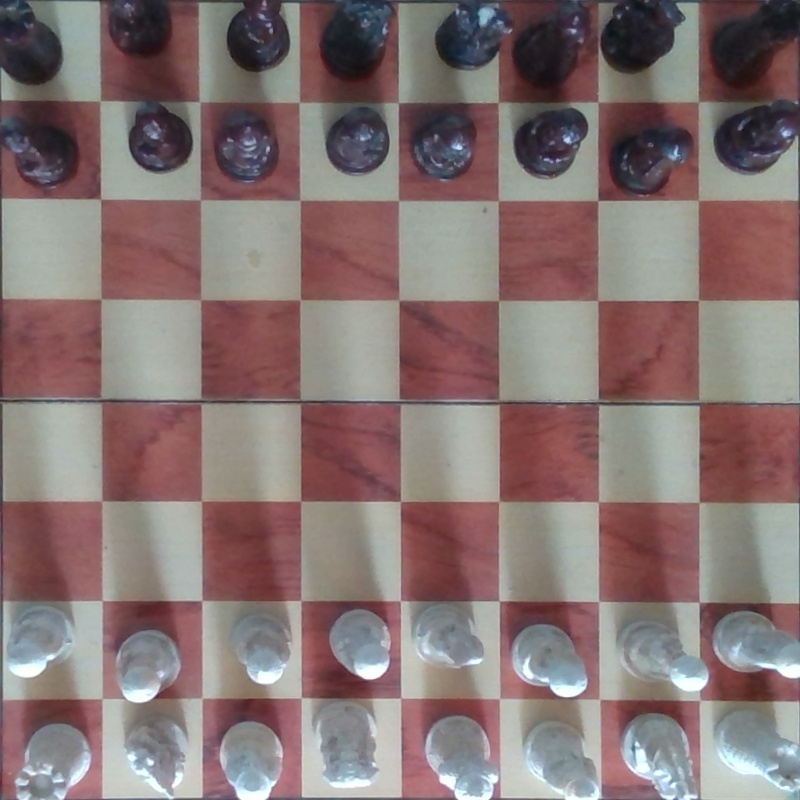
\includegraphics[width=0.19\textwidth]{trail_small_1.jpg} & 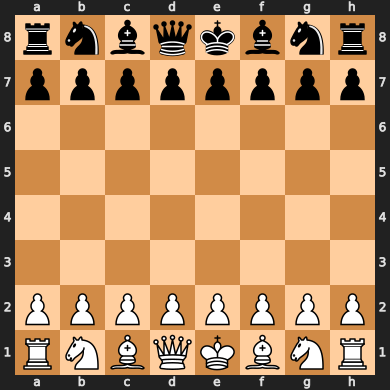
\includegraphics[width=0.19\textwidth]{starting_board.png} & 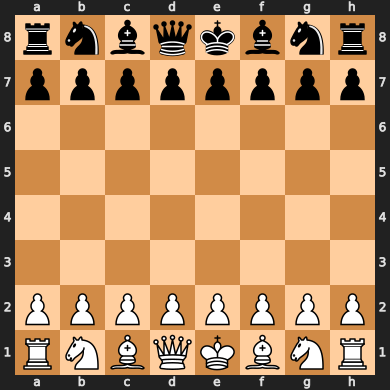
\includegraphics[width=0.19\textwidth]{starting_board.png} & 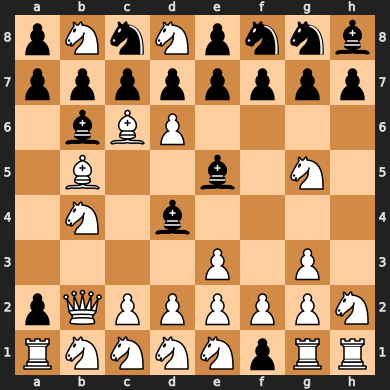
\includegraphics[width=0.19\textwidth]{mym_small_1.png} & 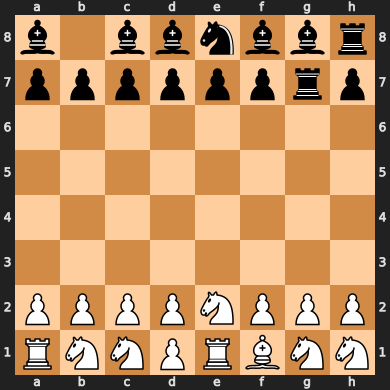
\includegraphics[width=0.19\textwidth]{cv_small_1.png} \\
        & Mistakes: & 0 & 12 & 3 \\
        \hline
        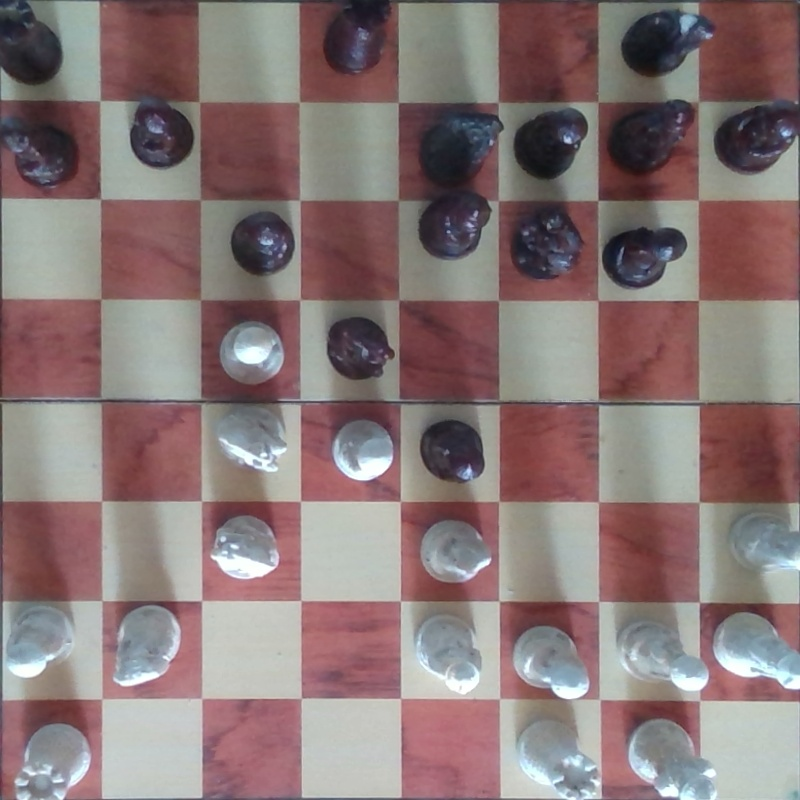
\includegraphics[width=0.19\textwidth]{trail_small_2.jpg} & 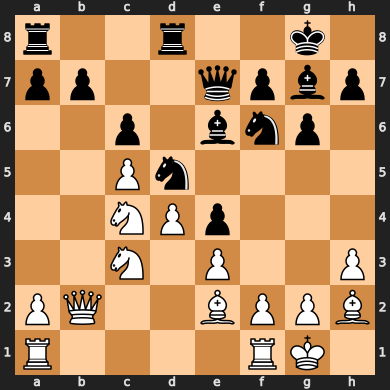
\includegraphics[width=0.19\textwidth]{small_board_2.png} & 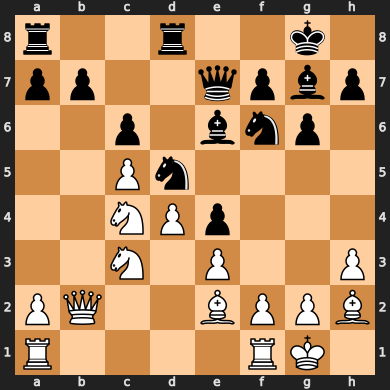
\includegraphics[width=0.19\textwidth]{small_board_2.png} & 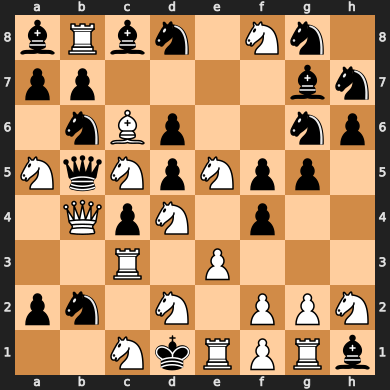
\includegraphics[width=0.19\textwidth]{mym_small_2.png} & 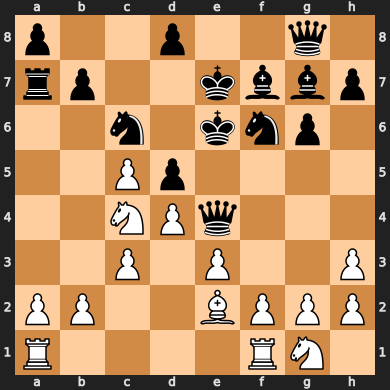
\includegraphics[width=0.19\textwidth]{cv_small_2.png} \\
        & Mistakes: & 0 & 12 & 3 \\
        \hline
        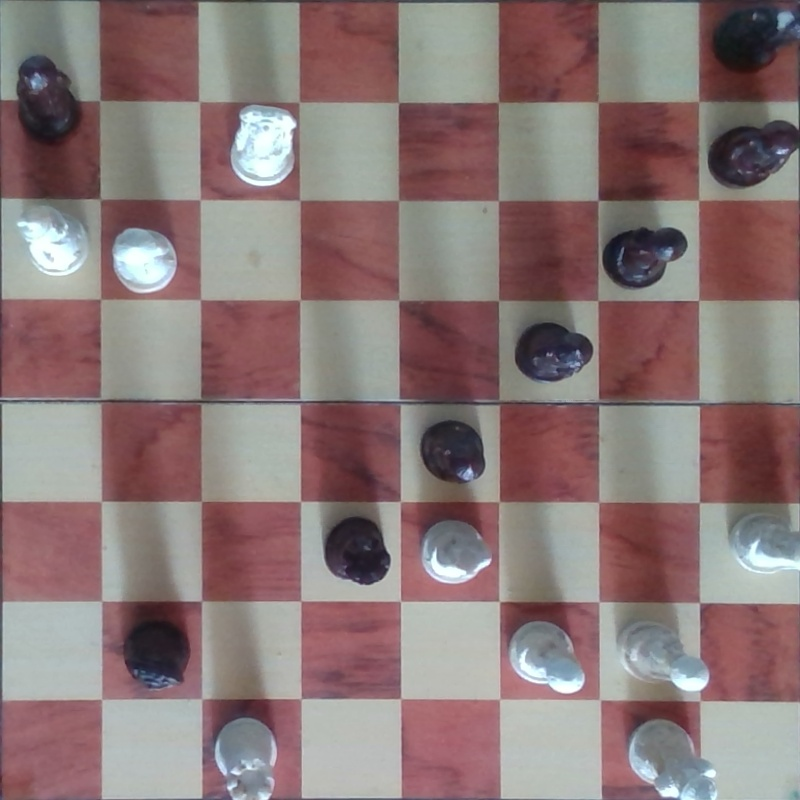
\includegraphics[width=0.19\textwidth]{trail_small_3.jpg} & 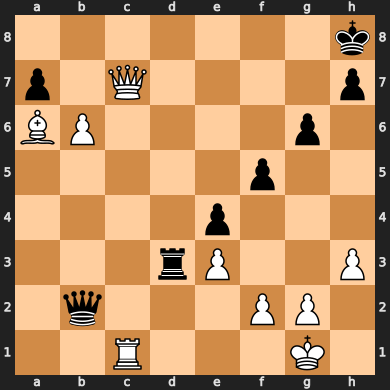
\includegraphics[width=0.19\textwidth]{small_board_3.png} & 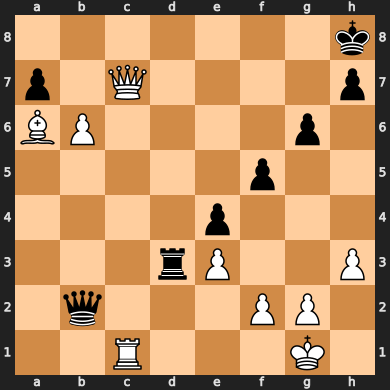
\includegraphics[width=0.19\textwidth]{small_board_3.png} & 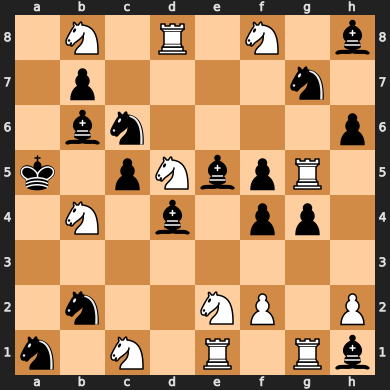
\includegraphics[width=0.19\textwidth]{mym_small_3.png} & 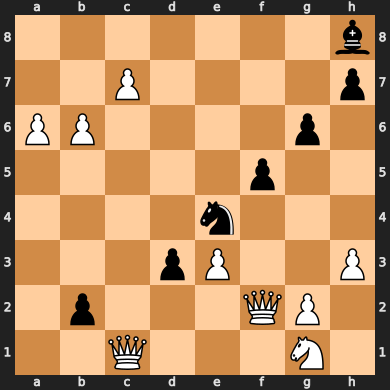
\includegraphics[width=0.19\textwidth]{cv_small_3.png} \\
        & Mistakes: & 0 & 12 & 3 \\
        \hline
        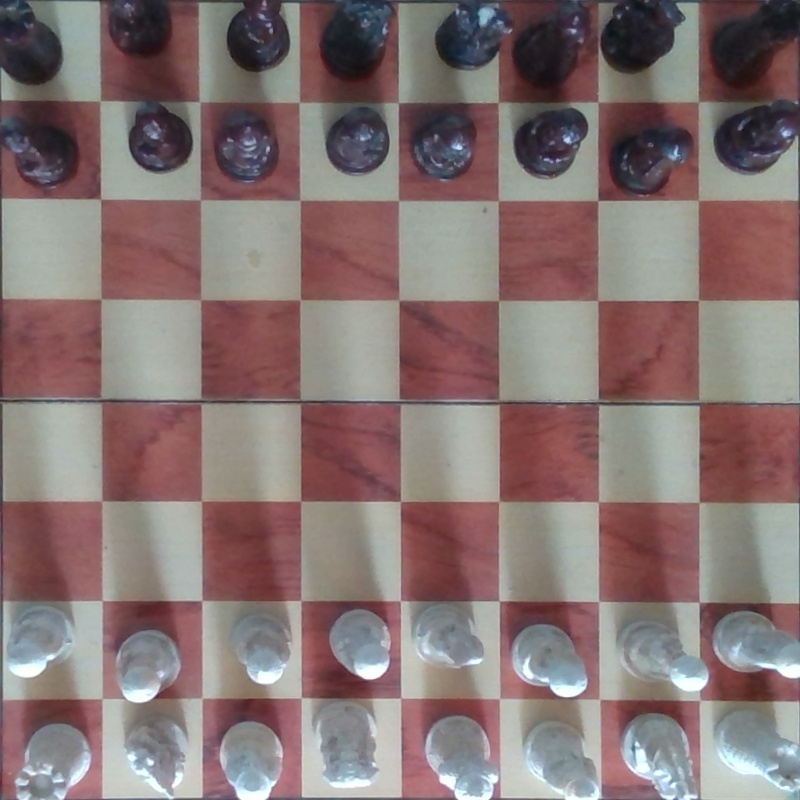
\includegraphics[width=0.19\textwidth]{trail_small_1.jpg} & 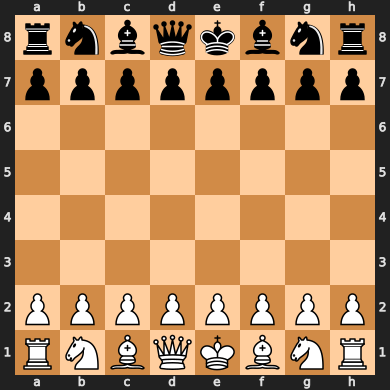
\includegraphics[width=0.19\textwidth]{starting_board.png} & 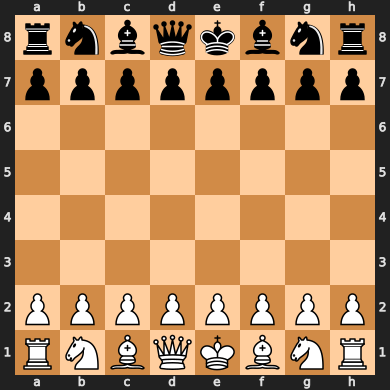
\includegraphics[width=0.19\textwidth]{starting_board.png} & 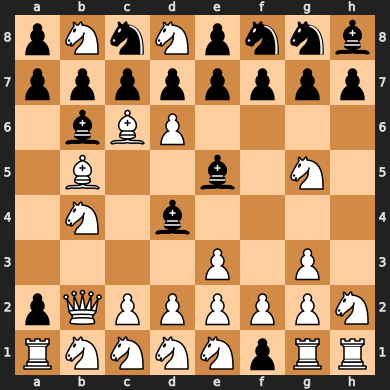
\includegraphics[width=0.19\textwidth]{mym_small_1.png} & 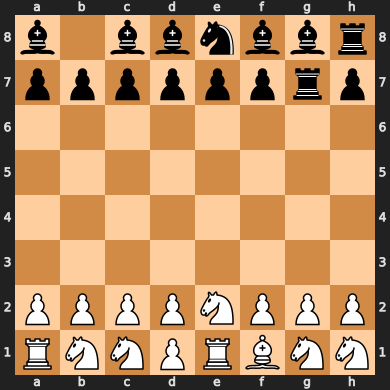
\includegraphics[width=0.19\textwidth]{cv_small_1.png} \\
        & Mistakes: & 0 & 12 & 3 \\
        \hline
        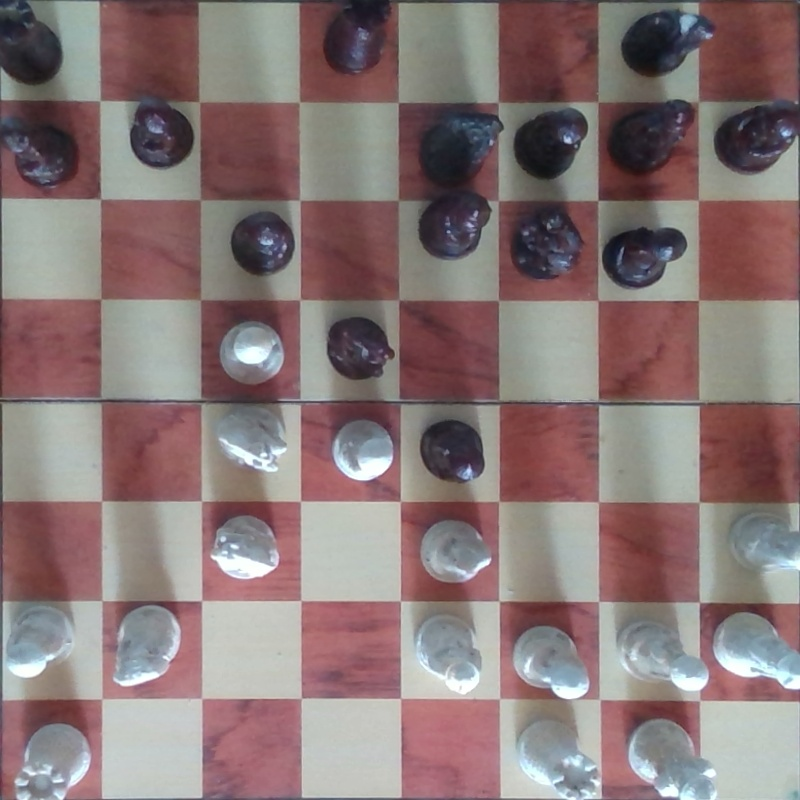
\includegraphics[width=0.19\textwidth]{trail_small_2.jpg} & 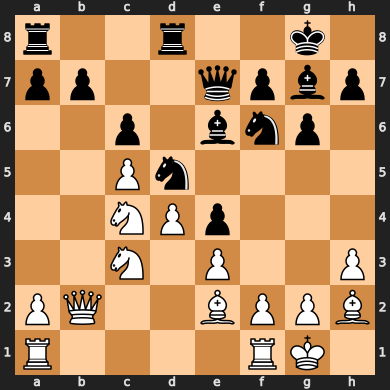
\includegraphics[width=0.19\textwidth]{small_board_2.png} & 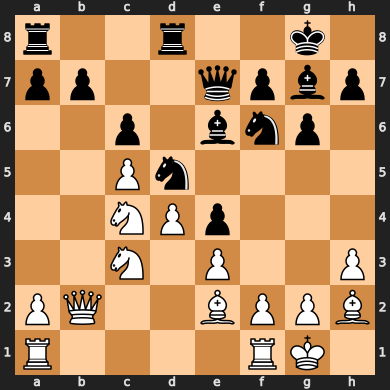
\includegraphics[width=0.19\textwidth]{small_board_2.png} & 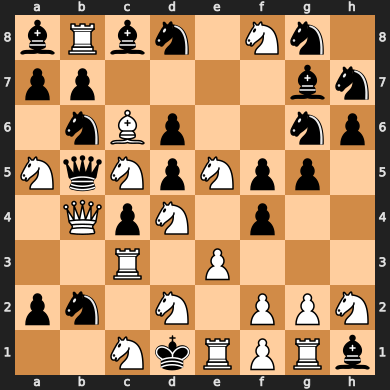
\includegraphics[width=0.19\textwidth]{mym_small_2.png} & 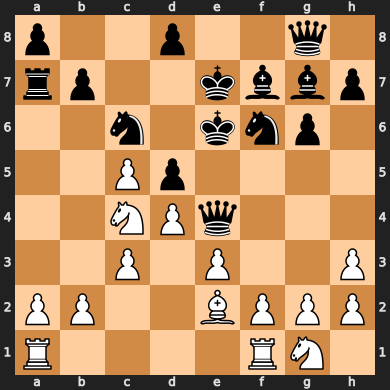
\includegraphics[width=0.19\textwidth]{cv_small_2.png} \\
        & Mistakes: & 0 & 12 & 3 \\
        \hline
        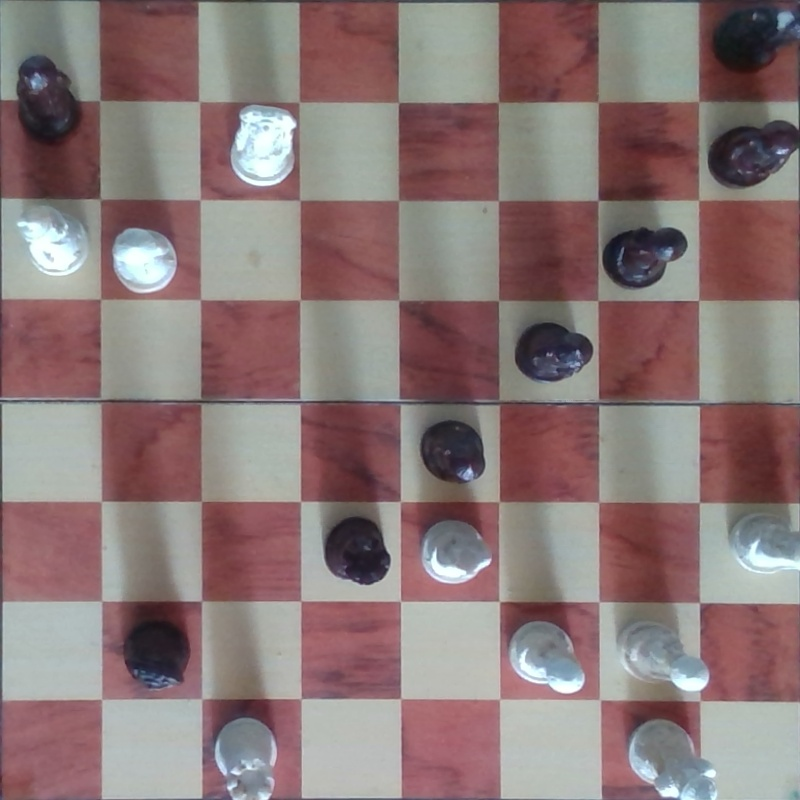
\includegraphics[width=0.19\textwidth]{trail_small_3.jpg} & 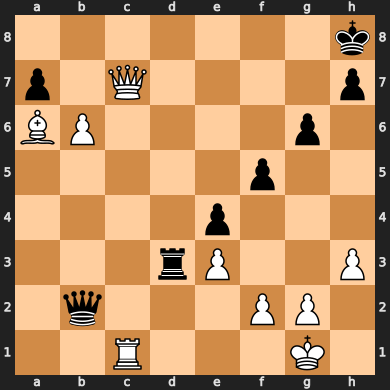
\includegraphics[width=0.19\textwidth]{small_board_3.png} & 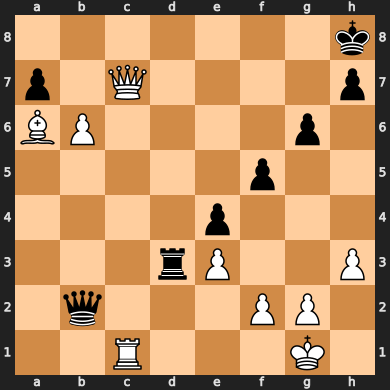
\includegraphics[width=0.19\textwidth]{small_board_3.png} & 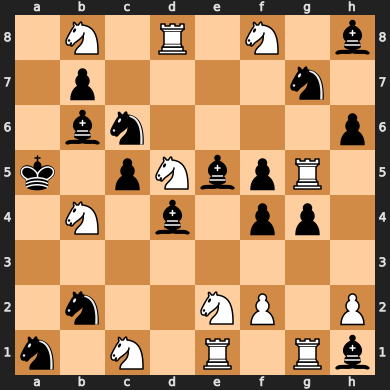
\includegraphics[width=0.19\textwidth]{mym_small_3.png} & 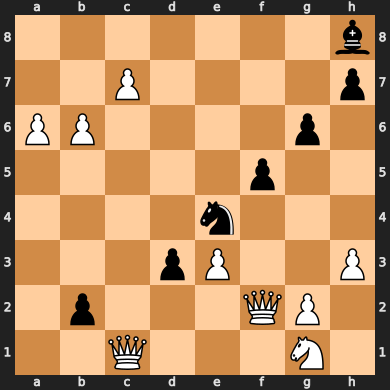
\includegraphics[width=0.19\textwidth]{cv_small_3.png} \\
        & Mistakes: & 0 & 12 & 3 \\
        \hline
    \end{tabu}}
}
\end{figure}


Talk about speed of inference and any other limitations of both presented and other work.

\section{Recording PGN}
\label{evaluate pgn}
In addition to evalutaing the raw model's performance, six games of varying length are played from beginning to end 
with the inference application.  
How well does it perform.  What did it take to get there?

\begin{figure}[h]
\centering
\begin{tabular}{|c|c|c|c|c|c|}
    \cline{4-6}
    \multicolumn{3}{c|}{} &  \multicolumn{3}{c|}{Delay for Move to Register (s)} \\
    \hline
    Game & Total Moves & PGN 100\% Correct & Median & Mean & Std Dev \\
    \hline
    Carlsen/Wesley & 57 & \checkmark & 1.25 & 3.01 & 5.26 \\
    Carlsen/Rapport & 36 & \checkmark & 1.13 & 3.21 & 4.97 \\
    Carlsen/Nakamura & 71 & - & 0.95 & 1.82 & 2.09 \\
    Carlsen/Aranian & 55 & \checkmark & 1.24 & 4.20 & 11.31 \\
    Fool's Mate & 4 & \checkmark & 0.95 & 1.19 & 0.76 \\
    \hline
\end{tabular}
\caption{Games played with the inference application}
\label{fig:games}
\end{figure}

The one failed game was due to the inference application registering a rook movement before the 
player lifted their hand from the rook and then decided to move it to a different square.

The fastest move to register took 0.27s and the slowest took 76s which appeared to be when there 
was lots of specular light reflecting from the pieces causing the model to confuse colors.

\begin{figure}[h]
    \centering
    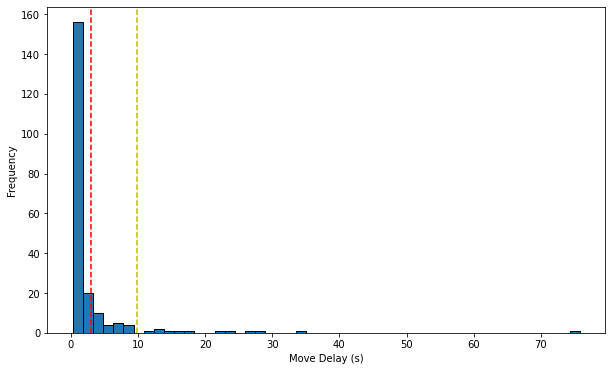
\includegraphics[scale=0.6]{move_delay.png}
    \caption{Histogram of move delay across all games in \autoref{fig:games} with arithmetic mean in red and sample standard deviation in yellow}
\label{fig:delay}
\end{figure}

How about performance?
Frames per second.  Analyse profiler.

\begin{figure}[h]
    \centering
    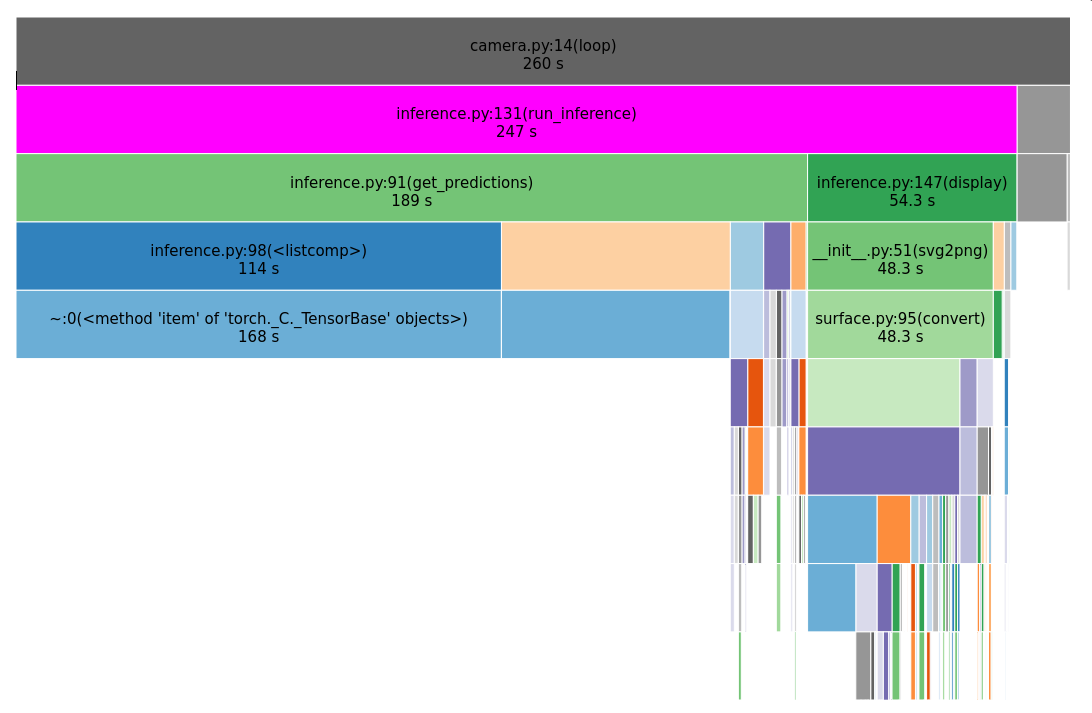
\includegraphics[width=\textwidth]{call_stack.png}
    \caption{cProfile Visualisation of recording a 4 minute game at inference with moves made in quick succession}
    \label{fig:profile}
\end{figure}